\documentclass[border=3pt]{standalone}
\usepackage[svgnames]{xcolor}
\usepackage{tikz}
\usetikzlibrary{positioning}
\usepackage{amsfonts}
\usepackage{pxfonts}

\newcommand{\N}{\ensuremath{\mathbb{N}} }% set of natural numbers
\newcommand{\Z}{\ensuremath{\mathbb{Z}} }% set of integers
\newcommand{\Q}{\ensuremath{\mathbb{Q}} }% set of rational numbers
\newcommand{\R}{\ensuremath{\mathbb{R}} }% set of real numbers
\newcommand{\C}{\ensuremath{\mathbb{C}} }% set of complex numbers
\renewcommand{\H}{\ensuremath{\mathbb{H}} }% set of hypercomplex numbers
\newcommand{\T}{\ensuremath{\mathbb{T}} }% set of transcendental numbers

\newcommand{\e}{\mathrm{e}}% exponential number

\newcommand{\definitions}{%
  % color of set of Natural numbers
  \colorlet{colN}{OrangeRed!60}
  % color of set of Integers
  \colorlet{colZ}{Orange!60}
  % color of set of Rational numbers
  \colorlet{colQ}{Gold!60}
  % color of set of Real numbers
  \colorlet{colR}{ForestGreen!50}
  % color of set of Complex numbers
  \colorlet{colC}{CornflowerBlue!80}
  % color of set of Hypercomplex numbers
  \colorlet{colH}{BlueViolet!50}
  % color of set of Transcendental numbers
  \colorlet{colT}{Green!30}

  % center coordinate of Natural numbers
  \coordinate (oN) at (0.0, 0.0);
  % center coordinate of Integers
  \coordinate (oZ) at (0.5, 0.5);
  % center coordinate of Rational numbers
  \coordinate (oQ) at (1.0, 1.0);
  % center coordinate of Real numbers
  \coordinate (oR) at (1.5, 1.5);
  % center coordinate of Complex numbers
  \coordinate (oC) at (2.0, 2.0);
  % center coordinate of Hypercomplex numbers
  \coordinate (oH) at (2.5, 2.5);
  % center coordinate of Transcendental numbers
  \coordinate (oT) at (0.5, 4.7);

  % set of Natural numbers
  \def\setN{(oN) ellipse (2.5 and 1.0)}
  % set of Integers
  \def\setZ{(oZ) ellipse (3.5 and 2.0)}
  % set of Rational numbers
  \def\setQ{(oQ) ellipse (4.5 and 3.0)}
  % set of Real numbers
  \def\setR{(oR) ellipse (5.5 and 4.0)}
  % set of Complex numbers
  \def\setC{(oC) ellipse (6.5 and 5.0)}
  % set of Hypercomplex numbers
  %\def\setH{(oH) ellipse (7.5 and 6.0)}
  % set of Transcendental numbers
  \def\setT{(oT) ellipse (1.5 and 0.67)}
}

\begin{document}
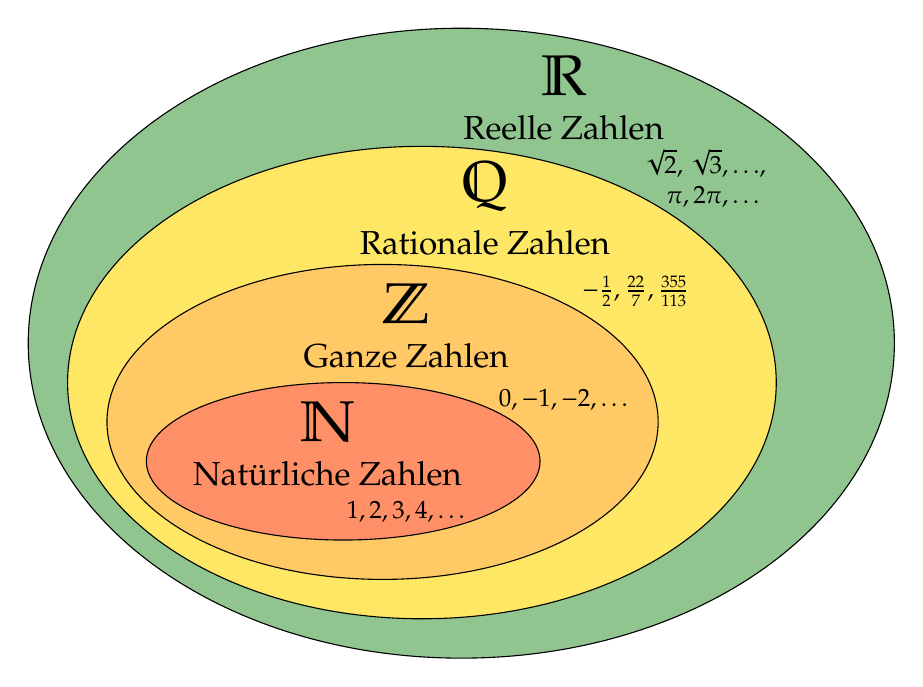
\begin{tikzpicture}
  
  % define colors and sets
  \definitions

  % fill sets in reverse order of size
  %\filldraw[fill=colH]\setH;
  %\filldraw[fill=colC]\setC;
  \filldraw[fill=colR]\setR;
  \filldraw[fill=colQ]\setQ;
  \filldraw[fill=colZ]\setZ;
  \filldraw[fill=colN]\setN;
  %\filldraw[fill=colT]\setT;

  % add set label for each set
  \node[font=\huge] (N) at (-.2, 0.5) {\N};
  \node[font=\huge] (Z) at (0.8, 2.0) {\Z};
  \node[font=\huge] (Q) at (1.8, 3.5) {\Q};
  \node[font=\huge] (R) at (2.8, 4.9) {\R};
  %\node[font=\huge] (C) at (3.8, 6.3) {\C};
  %\node[font=\huge] (H) at (4.8, 7.8) {\H};
  %\node[font=\large] (T) at (0.8, 4.9) {\T};

  % add name label for each set
  \node[font=\large] [below=0ex of N] {Natürliche Zahlen};
  \node[font=\large] [below=0ex of Z] {Ganze Zahlen};
  \node[font=\large] [below=0ex of Q] {Rationale Zahlen};
  \node[font=\large] [below=0ex of R] {Reelle Zahlen};
  %\node[font=\large] [below=0ex of C] {Complex};
  %\node[font=\large] [below=0ex of H] {Hypercomplex};
  %\node[font=\small] [below=-1ex of T] {Transcendental};

  % add number examples for each set
  \node[font=\small] [below right=3ex and -1em of N] {$1,2,3,4,\ldots$};
  \node[font=\small] [below right=3.5ex and 1.8em of Z] {$0, -1, -2, \ldots$};
  \node[font=\small] [below right=3.5ex and 2em of Q] {$-\frac{1}{2},\frac{22}{7},\frac{355}{113}$};
  \node[font=\small,align=left] [below right=2.6ex and 1.3em of R] {$\sqrt{2},\sqrt{3},\ldots$,\\ \quad$\pi,2\pi,\ldots$};
  %\node[font=\small] [below right=3.5ex and 1em of C] {$\sqrt{-1},i,\sqrt{i},\e^{i}$};
  %\node[font=\small] [below right=3.5ex and -1em of H] {Hypercomplex};
  %\node[font=\small] [below=1ex of T] {$\pi,\e,\gamma$};

\end{tikzpicture}
\end{document}
